\subsection{Restoring layers}
\label{sec:restore-desgin}
%\paragraph{Parallel slice restoring}
%\label{subsubsec:slice-restoring}



\begin{figure}[t]
	\centering
	\centering
	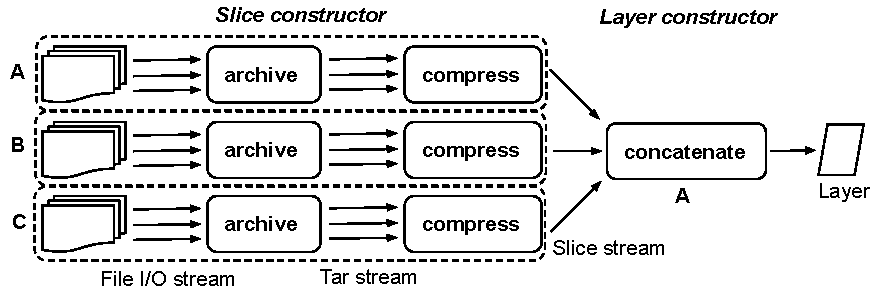
\includegraphics[width=\columnwidth]{graphs/sift-layer-construct-new.pdf}
	\caption{Parallel streaming layer construction.}
	\label{fig:construct}
\end{figure}



%When a~\texttt{pull} layer request is received and its associated 
%P-servers fail, D-servers will rebuild a layer for the request.
%\sysname will first search layer preconstruct cache on D-servers.
%If not found,
%\sysname will rebuild the layer according to the layer recipe. 
%the \dedupname~system 
%first prepares a directory structure for the slice, based on the slice recipe.
%Then, it copies the files into the directory tree.
%Next, it compresses the slice's directory tree into a slice tarball,
%and directly sends it back to the client.

%\LR{Are we only considering the case when a P-server fails or
%are we also considering, if a P-server gets overloaded?}

To restore a layer, each D-server in \sysname has a slice constructor and
layer constructor. The restoring process works as follows:

First, the layer constructor fetches the layer recipe from metadata database.
As shown in Figure~\ref{fig:construct}, according to $L1$'s layer recipe, 
the restoring workers are D-server $A$, $B$, and $C$.
Since $A$ is the restoring master \LR{Explain how the master is picked},
it sends \texttt{GET slice} requests for their primary slices to $B$ and $C$.
Note that the master first tries to rebuild the layer from primary slices.
If a primary slice is missing, the master will find its corresponding backup
slice and send a \texttt{GET slice} request to the corresponding D-server.

%\paragraph{Parallel slice construction}

%Upon a \texttt{pull} layer request fails on P-servers,
%\sysname initiates a layer restoring process on D-servers for it.
%which involves two modules: slice constructor and layer constructor. 

After a \texttt{GET slice} request has been received, 
$B$ and $C$'s slice constructors start rebuilding their primary slices and send them to $A$.
Meanwhile $A$ instructs its local slice constructor to restore its primary slice for $L1$.
%
To construct a layer slice, a slice constructor first gets the associate slice recipe
from the metadata database. The recipe is keyed by a combination of layer Id, host address and requested
backup level, i.e., \emph{L1::A::}\texttt{P} \LR{More details here. Why is that they key? Why is the backup
level relevant?}.
Then, the slice constructor creates a slice tar archive by writing each file header and the corresponding
file content from the slice recipe.
%rebuilds each file entry in the slice tar archive according to the slice recipe.

\paragraph{Optimizations}
The layer restoration performance is critical to keep \texttt{pull} latencies low. Hence,
\sysname uses several optimiations to streamline the process.
%
Besides parallelizing layer reconstruction across D-servers, \sysname also
parallelizes slice reconstruction on a single node.
%
Additionally, \sysname avoids generating intermediate files on disk to reduce disk I/O.
%
%To avoid generating any intermediate files stored on disk to reduce disk I/Os
%and improve restoring performance, the slice restoring process is a stateless streaming
%slice construction process.
%
%All the involved data processing operations are preceded in memory as streaming. 

Specifically, a slice constructor first reads each entry in the slice recipe
and gets each header and its corresponding content pointer.
%
Then, the slice constructor reads the corresponding physical files addressed by the content
pointers in parallel from the D-server's file store.
%
\LR{The following is unclear. What does ``asynchronously'' mean in this case? Is every
file written to its own buffer in parallel and then combined in a single archive buffer?}
Each file is written to a slice archive buffer asynchronously.
Before writing file content to the archive buffer, slice constructor first writes its
associated file header into the archive buffer according to the slice recipe.

After archiving all the files along with their headers in the slice archive buffer,
the archive buffer will be divided into several chunks, compressed in parallel,
and concatenated into a single compressed slice.
%
%Then, it writes the header in the slice archive.
%After that it put the associated file content in the slice archive
%by reading the corresponding physical file addressed by the content pointer.
%fetches files pointed by content
%and builds a slice archive.
%
%Next, the slice constructor sends the slice stream to the layer constructor on restoring master
%via network.

%first, slice constructor loads file in parallel from file store based on the slice recipe.
% along with their corresponding headers saved in slice recipe.

%\LR{The following paragraph is a little bit out of context. Why are we suddenly talking about
%stateless streaming layer construction? Need to tie it in better with the rest of the text and
%motivate our design decisions better.}

%\paragraph{Streaming layer construction}
\LR{What exactly do you mean by ``Through network transfer''? Are the different slices kept inmemory at the master for concatenation after they have been received?}
Through network transfer, multiple compressed slices will be concatenated into a single
layer compressed tarball and sent back the client as shown in Figure~\ref{fig:construct}.
As a result no intermediate file will be created or stored on disk. % subil: whoa!
%After receiving all slices, layer constructor on \emph{A} will concatenate all slices into a compressed layer
%. 
%Overall, the layer restoring process is a stateless streaming layer construction process.
%
%All the involve data processing operations are preceded in memory as streaming 
%without creating any intermediate files stored on disk to reduce disk I/Os and improve
%performance.

Furthermore, \sysname also provisions a small in-memory file cache on each D-server to cache hot files.
This reduces disk I/O during restoration even further. The file cache uses Adaptive
Replacement (ARC)~\cite{xxx} \todo{fill in more details on how the cache works, how big it is, etc.}
%
\LR{It would be good to have a graph in the evaluation, showing how each of those optimizations
reduces reconstruction time.}

%headers according to $Dests$,
%after that it writes file contents into the archive
 
%Slice restoring process has four suboperations: 
%slice recipe lookup,
%slice file copying,
%slice compression, and
%slice network transfer. 
%To measure the overhead for each suboperation, 
%we implemented layer deduplication and parallel slice
%restoring on a 4-node registry cluster. 
%We first warmup the cluster by pushing 200 layers to the cluster
%and initiating layer deduplication process.
%The layers were randomly selected from our layer dataset detailed in xxx limited to 50MB.
%After finishing layer deduplication,
%we sent 400 \texttt{pull slice} requests to the cluster with 10 \texttt{pull slice} requests issued at a time.
%Figure~\ref{fig:slice-restoring-breakdown} shows the CDFs of the latencies for each suboperation.
%We see that across the four suboperations,
%the duration for slice compress is the shortest.
%Slice compression only took less than 0.001 s because a slice is a smaller unit. 
%The next shortest suboperation is network transfer since we pulled layer slice through Ethernet.
%90\% of slice recipe lookups took less than 0.1 s while 
%the highest slice recipe lookup duration almost reaches 0.8 s,
%which is caused by high concurrent lookup requests 
%%(note that we use redis to store metadata \NZ{use mongodb instead}).
%The most time consuming suboperation is slice file copying, which involves 
%copying all 
%the files that belong to the slice to their destination directory based on the slice recipe.
%Note that we implemented a thread pool on each registry server to read files in parallel
%and write data in RAMdisk to reduce disk IOs.
%40\%of slice file copying duration is greater than 1 s and 
%10\% of slice file copying duration is higher than 10 s.
%This is because bigger slices contains more files and requires more disk IOs.
%The overhead of slice copying can be largely mitigated for a large-scale registry cluster
%since the size of slice roughly equals to $S_{l}/N$, where $S_{l}$ denotes the layer size and $N$ is size of registry cluster.
%However, it could be a bottleneck for slice restoring on a small-scale registry cluster.
%%and slice file copying duration depends on slice size.
%
%%\begin{algorithm}
\scriptsize 
	\caption{File cache assisted slice restoring}
	\label{alg:file-cache}
	\KwIn{\\
		$\theta_{rsfc}$: Slice restoring latency threshold. \\
		$s$: Slice to be restored. \\
	}

	\SetKwFunction{Fsub}{Restore}
	\SetKwProg{Fn}{Function}{:}{}

	\Fn{\Fsub{s}}{
		%{\tiny\texttt{/* Otherwise, it's a repull layer miss   /}}\\
		\eIf{files in s are cached in file cache}
		{
			slice $\gets$ \texttt{RestoreSlice} \emph{s} \texttt{From} \emph{file cache + disk} 
		}
		{
			slice, $D_{rs}$ $\gets$ \texttt{RestoreSlice} \emph{s} \texttt{From} \emph{disk} \\
			\If{ $D_{rs} > \theta_{rsfc}$} 
			{ 
				\emph{file cache} $\gets$ \texttt{Cache} \texttt{Subsetof} \emph{s.files}
			}		
		}
	}

\end{algorithm}



%
%To reduce slice file copying overhead,
%\sysname~\filecachename~temporally cache a subset of unique files for bigger and popular slices that have a high slice restoring latency, ie., $D_{rs} > \theta_{rsfc}$, 
%where $D_{rs}$ is the slice restoring latency and $\theta_{rsfc}$ is the restoring latency threshold for 
%caching
%a subset of files from the slice to help improve its restoring performance as shown in Algorithm~\ref{alg:file-cache}.
%Upon a \texttt{pull slice} request for those slices, 
%\dedupname~ system fetches a subset of its containing files from \filecachename~and
%the remaining files from disk for slice restoring.
%
%To identify which slices have a high slice restoring latency,
%\dedupname~system monitors slice restoring performance and 
%maintains a restoring performance  profile for each slice that has been restored,
%% as shown in Figure~\ref{fig:xxx},
%which contains the latency breakdown of slice restoring
%% (,and a decompression latency updated by layer decompression process) 
%and its containing files' sizes.
%All the slice restoring performance profiles are also stored in distributed  databases,
% and addressed by slice digests. 
%To estimate the restoring latency for a slice $i$ that hasn't been restored, 
%\dedupname system~first lookups the slice restoring performance profiles by slice size,
% then selects a slice $x$ that is most similar in size to $i$,
% and estimates $i$'s restoring latency as: 
% $D_{rs}(i) \approx D_{rs}(x) + \Phi_{rs}(\Delta_{S})$,
% where $\Delta_{S}$ is the size different between two slices.
% $\Phi_{rs}(\Delta_{S})$ denotes a slice restoring latency function of slice size variation.
%  $\Phi_{rs}(\Delta_{S})$ is generated by using linear regression~\cite{xxx}.
% %$\varepsilon_{rs}$ is the standard error of restoring latency estimation for the layers similar in size.
%If the estimated slice restoring $D_{rs}(i) > \theta_{rs}$,
%then, \dedupname~lookups the slice restoring performance profiles by slice size,
%selects a slice $y$ that has a acceptable restoring latency and
%most similar in size to $i$.
%Next, \dedupname system~caches a subset of files $F$ for slice $i$, so that
%$D_{rs}(i) - \Phi_{rs}(\Sigma_{S}(F)) \approx D_{rs}(y)$,
%where $\Sigma_{S}(F)$ is the sum size of files in $F$.
%
%Note that \filecachename~size is limited so that \filecachename~only caches 
%subsets of files for big slices that belongs to popular layers.
%%that will be accessed later. 
%\cref{sec:cache-design} will describe how to determine popular layers based on user access patterns.
%Note that the slices for the same layer have similar sizes, restoring latencies, and popularity 
%because of unique file
%distribution. 
%Thus, once a layer is determined as popular layer, 
%\dedupname~will cache similar amount of files for its slices.
%Note that all the files in file cache are unique and can be shared for restoring different slices.
%
%For on-premise or private registry cluster, the network transfer speed is usually faster than remote cloud.
%Thus, slice compression is less important for medium to small size slices, 
%especially for the slices that have a high decompression latency, 
%i.e., $D_{stt} < \theta_{stt}$ and $D_{dc} > \theta_{dc}$, where $D_{stt}$ and $D_{dc}$ denote slice transfer duration
%and decompression duration respectively; 
%$\theta_{stt}$ and $\theta_{dc}$ denote thresholds for them respectively.
%Consequently, \dedupname system~only archives these slices without compressing them and directly sends
%these archival files back to the clients to eliminate clients' decompression latency.



%}